\documentclass[a4paper,12pt,french]{article}

\usepackage[cours]{../../../Style}

%\selectcolormodel{cmyk}

%\usepackage{wrapfig}

% Début du document
%%%%%%%%%%%%%%%%%%%
\begin{document}

\title{Dérivation}
\maketitle

\begin{programme}
\item Fonction dérivée
\item Dérivées de $x \mapsto x^2$, $x \mapsto x^3$, de combinaisons linéaires, de polynômes de degré $\leq 3$
\item Sens de variation d'une fonction, lien avec le signe de la dérivée
\item Tableau de variations, extremums
\item Capacités
\begin{itemize}
\item Calculer la dérivée d'un polynome de degré $\leq 3$
\item Déterminer le sens de variation et les extremums d'une fonction polynome de degré $\leq 3$
\end{itemize}
\end{programme}

\section{Généralités, règles de calcul}

\begin{defin}
On définit la fonction dérivée de $f$, notée $f'$, qui à $x$ associe le coefficient directeur de la tangente à la courbe de $f$ au point d'abscisse $x$.
\end{defin}

\begin{prop}
On a les dérivées usuelles suivantes:
\begin{center}\renewcommand{\arraystretch}{1.5}
\begin{tabularx}{5cm}{|Y|Y|} \hline
$f(x)$ & $f'(x)$ \\ \hline
$k \in \R$ & $0$ \\ \hline
$x$ & $1$ \\ \hline
$x^2$ & $2x$ \\ \hline
$x^3$ & $3x^2$ \\ \hline
\end{tabularx}
\end{center}
\end{prop}


\begin{prop}
Soient $f$ et $g$ deux fonctions, et $k \in \R$. Alors:
\begin{itemize}
\item $(f+g)'=f'+g'$
\item $(k f)'=k f'$
\end{itemize}
\end{prop}

\begin{exs}
\begin{itemize}
\item Soit $f:x \mapsto {\color{DarkRed}x^2}+{\color{DarkBlue}2x}+{\color{black}1}$. Alors $f'(x)={\color{DarkRed}2x}+{\color{DarkBlue}2 \times 1} + {\color{black}0} =2x+2$.
\item Soit $g:x \mapsto x^3-3x-2$. Alors $f'(x)=3x^2-3$.
\item Soit $h:x \mapsto x^2+x^2$. Alors $f'(x)=2x+2x=4x$.
\end{itemize}
\end{exs}

%$f(x)=\tikzmark{cube} \ 2x^{\tikzmark{expcube} 3}-\tikzmark{carre}3x^{\tikzmark{expcarre} 2}+5\cancel{x} \cancel{-1}$

%\tikz[remember picture]{\draw[overlay,->] (pic cs:expcube) to[bend right=80] (pic cs:cube);}
%\tikz[remember picture]{\draw[overlay,->] (pic cs:expcarre) to[bend right=10] (pic cs:carre);}

\section{Lien avec les variations}

\begin{thm}
Soit $f$ une fonction et $a \in \R$, $b \in \R$.
\begin{itemize}
\item Si $f'$ est positive sur $[a;b]$, alors $f$ est croissante sur $[a;b]$.
\item Si $f'$ est négative sur $[a;b]$, alors $f$ est décroissante sur $[a;b]$.
\item Si $f'$ est nulle sur $[a;b]$, alors $f$ est constante sur $[a;b]$. Les zéros de $f'$ correspondent aux \textbf{extremums locaux} de $f$ (les \og sommets \fg).
\end{itemize}
\end{thm}

\begin{app}
On peut alors dresser le tableau de variations d'une fonction grâce au tableau de signes de sa dérivée.
\end{app}

\begin{ex}
\compo[0.52]
{\setlength{\parskip}{1ex}
Soit $f:x \mapsto x^2-4x+2$. Alors $f'(x)=2x-4$.

On a $f'(x)=0$ ssi $2x=4$ ssi $x=2$. (On peut aussi calculer $\frac{-b}{a}$).

On a de plus $f(2)=2^2-4 \times 2+2=4-8+2=-2$.

Cela donne alors:
}
{
\begin{centrer}
\begin{tikzpicture}
\tkzTabInit[lgt=1.5,espcl=2.2]{$x$ /1, $f'(x)$/1, $f(x)$/2}{$- \infty$, $2$, $+ \infty$}
\tkzTabLine{,-,z,+}
\tkzTabVar{+/$ $, -/$-2$, +/$ $}
\end{tikzpicture}
\end{centrer}
}
\end{ex}
\end{document}
